\documentclass[12pt]{article}

\usepackage{amsmath,amssymb}
\usepackage{graphicx}
\usepackage{geometry}
\usepackage{setspace}
\usepackage{natbib}
\usepackage{hyperref}
\usepackage{booktabs}

\geometry{margin=1in}
\doublespacing
\graphicspath{{figures/}}

\newcommand{\ShortTitle}{Sulcal dipole slowing in mechanistic CSD}
\newcommand{\TOCSummary}{A multi-ion surface electrodiffusion model predicts that sulcal dipole alignment adds a significant, fold-dependent slowing term on top of extracellular diffusion.}

\title{Sulcal dipole alignment slows cortical spreading depolarization in a mechanistic surface electrodiffusion model}

\author{
Antonio Pereira\thanks{Correspondence: Antonio Pereira, \texttt{apereira@ufpa.br}; ORCID: 0000-0002-0808-1058.}\\
\small Institute of Technology, Federal University of Para (UFPA)
\and
Rubem Guedes\\
\small Department of Nutrition, Federal University of Pernambuco (UFPE)\\
\small \texttt{guedes.rca@gmail.com}; ORCID: 0000-0002-2396-4019
}

\date{}

\begin{document}
\maketitle

\begin{center}
\parbox{0.95\textwidth}{\small
\textbf{Condensed title:} \ShortTitle\\
\textbf{Summary:} \TOCSummary}
\end{center}

\begin{abstract}
Cortical spreading depolarization (CSD) slows in sulci, but the mechanism of that slowing is still debated because scalar attenuation models, tensor transport models, and electrodiffusive models emphasize different aspects of cortical folding. We asked whether sulcal dipole alignment can impose a measurable additional delay in a mechanistic surface model that keeps extracellular diffusion central while representing ionic drift and membrane charge separation explicitly. We implemented a folded-surface electrodiffusion model with overlapping extracellular and intracellular compartments, explicit extracellular and intracellular K$^+$, Na$^+$, and Cl$^-$ concentrations, Goldman--Hodgkin--Katz membrane voltage, leak and activation-dependent membrane currents, Na/K pump dynamics, dynamic extracellular-space volume fraction and tortuosity, and a quasi-static dipole-driven extracellular potential field aligned to local surface normals. We then compared the same mechanistic model with dipole alignment disabled or enabled across one representative folded surface and a paired geometry sweep spanning 12 folded surfaces plus a flat control. In the representative folded case, cross-fold propagation slowed from 2.488 to 2.106~mm/min when the dipole term was enabled, while cross-fold delay increased from 134.4 to 159.2~s. Across the full sweep, all 12 folded geometries slowed with dipole alignment, whereas the flat control was unchanged. The mean dipole-induced slowdown was 0.243~mm/min (95\% bootstrap confidence interval 0.208--0.276~mm/min), corresponding to a 9.08\% reduction in speed and a mean delay increase of 13.46~s (95\% confidence interval 12.25--14.65~s). Paired Wilcoxon signed-rank tests were significant for cross-fold speed ($p=2.44\times 10^{-4}$), cross-fold delay ($p=2.44\times 10^{-4}$), and deep-edge local speed ($p=2.44\times 10^{-3}$). Slowdown increased strongly with fold depth (Spearman $\rho=0.95$, $p=2.25\times 10^{-6}$). These results support a mechanistic interpretation in which extracellular diffusion remains the backbone of propagation, but sulcal dipole alignment adds a significant, geometry-specific electrodiffusive slowing term that is absent on a flat surface.
\end{abstract}

\noindent \textbf{Keywords:} cortical spreading depolarization, electrodiffusion, sulcus, extracellular diffusion, dipole alignment, cortical folding, surface model

\section{Introduction}

Cortical spreading depolarization (CSD) is a propagating wave of near-complete cellular depolarization that travels through cortex at millimeters per minute and is implicated in migraine aura, ischemic injury, and traumatic brain injury \citep{Pietrobon2014,Ayata2015,Woitzik2013,Dreier2017}. The effect of cortical folding on CSD propagation remains difficult to isolate because sulci alter extracellular geometry, tissue orientation, and the alignment of current sources simultaneously. As a result, a slower wave in the sulcus can be interpreted as reduced effective coupling, altered preferred transport orientation, or a field-mediated electrodiffusive effect.

Earlier modeling work in this repository addressed that question using scalar attenuation fields and orientation-aware tensor transport. Those studies were useful for showing that sulcal slowing survives when directional structure is represented explicitly, but they did not resolve ionic concentrations, extracellular charge redistribution, or dynamic extracellular-space (ECS) restriction. That limitation matters because the CSD literature consistently places extracellular ionic diffusion, homeostatic membrane fluxes, and ECS geometry at the center of propagation \citep{Tuckwell1978,Wei2014,Zandt2015}. In that literature, the electrical component is typically represented not as propagating electromagnetic radiation, but as quasi-static extracellular potential generated by membrane currents and ionic concentration gradients.

The present study therefore asks a more mechanistic question: if extracellular diffusion remains the backbone of propagation, does sulcal dipole alignment impose an additional slowing term when ionic drift, membrane voltage, pump dynamics, and ECS swelling are represented explicitly on a folded cortical surface? Our working hypothesis is that sulcal dipole alignment should be specific to folded geometries, negligible on a flat control, and stronger in deeper or narrower folds because those geometries increase the alignment between membrane-current source orientation and the cross-sulcus propagation path. That hypothesis is motivated by the general principle from EEG/MEG forward modeling that cortical folding and dipole orientation strongly shape mesoscale extracellular fields \citep{Ahlfors2010a,Ahlfors2010b,Muller2023,Reimann2022}, but here it is tested against CSD propagation rather than observability.

\section{Materials and methods}

\subsection{Synthetic cortical-surface geometry}

We used a triangulated folded-strip surface to isolate sulcal geometry while keeping the model computationally tractable. The representative surface contained 1,792 vertices and 3,402 triangular faces over a 22~mm by 10~mm domain, with a central sulcal depression generated by a Gaussian fold profile of depth 2.4~mm and width parameter $\sigma=1.5$~mm. Each vertex carried normalized sulcal-depth, thickness, and vascular-risk fields derived from the synthetic geometry. A tangential preferred-axis field followed the long axis of the folded strip. The geometry sweep used 12 folded surfaces with depths 1.2, 1.8, 2.4, and 3.0~mm crossed with width parameters $\sigma \in \{1.1,1.5,1.9\}$~mm, plus a flat control with zero fold depth.

Propagation was initiated by a focal stimulus placed on one sulcal bank. Arrival time was then measured at two automatically selected electrode regions on opposite banks. The primary readout was the cross-fold propagation speed inferred from the geodesic distance between the electrode regions and the difference between their median arrival times. This metric is directly analogous to the inter-electrode timing readouts reported in invasive CSD studies \citep{Dreier2017}.

\subsection{Mechanistic surface electrodiffusion model}

The surface model evolves explicit extracellular and intracellular concentrations of K$^+$, Na$^+$, and Cl$^-$ on overlapping surface compartments. For each ionic species $s \in \{\mathrm{K},\mathrm{Na},\mathrm{Cl}\}$, the extracellular concentration $c_s^{e}$ obeys
\begin{equation}
\frac{\partial c_s^{e}}{\partial t}
= \nabla_{\Gamma}\cdot\left[D_s(\alpha,\lambda)\left(\nabla_{\Gamma} c_s^{e} + z_s \beta_{\mathrm{ed}} c_s^{e}\nabla_{\Gamma}\phi\right)\right]
 \frac{J_s^{m}}{\alpha},
\end{equation}
where $\Gamma$ is the cortical surface, $\alpha$ is local ECS volume fraction, $\lambda$ is tortuosity, $z_s$ is ion valence, $D_s$ is the effective surface diffusivity, $\beta_{\mathrm{ed}}$ is the electrodiffusion gain, and $J_s^{m}$ is the membrane source term. The intracellular compartment is updated by mass conservation,
\begin{equation}
\frac{\partial c_s^{i}}{\partial t} = -\frac{J_s^{m}}{1-\alpha}.
\end{equation}
Effective extracellular diffusion was scaled by $\alpha/\lambda^2$, so deeper and more swollen tissue automatically restricted diffusion more strongly.

Membrane voltage was updated from a Goldman--Hodgkin--Katz relation using dynamic ionic concentrations and activation-dependent permeabilities. Leak and activated membrane currents were represented by conductance-based terms referenced to the Nernst potentials of K$^+$, Na$^+$, and Cl$^-$. The Na/K pump depended on intracellular Na$^+$, extracellular K$^+$, and, in the vascular sensitivity analysis, local oxygen:
\begin{equation}
P_{\mathrm{pump}} = P_{\max} f_{\mathrm{Na}}(c_{\mathrm{Na}}^{i}) f_{\mathrm{K}}(c_{\mathrm{K}}^{e}) f_{\mathrm{O}_2}(O).
\end{equation}
An activation variable $\theta$ evolved sigmoidally as a function of extracellular K$^+$ and membrane voltage and controlled the transition between resting and depolarized membrane conductances.

The extracellular electrical field was treated quasi-statically. Charge-density deviations from rest were defined as
\begin{equation}
\rho_e = (c_{\mathrm{K}}^{e}-c_{\mathrm{K},0}^{e}) + (c_{\mathrm{Na}}^{e}-c_{\mathrm{Na},0}^{e}) - (c_{\mathrm{Cl}}^{e}-c_{\mathrm{Cl},0}^{e}),
\end{equation}
and the potential field $\phi$ was obtained from a screened surface equation,
\begin{equation}
-\nabla_{\Gamma}\cdot(\sigma_{\phi}\nabla_{\Gamma}\phi) + \kappa \phi
= \gamma_{\rho}\rho_e - \gamma_{d}\mathcal{K}_{d}[I_m],
\end{equation}
where $\sigma_{\phi}$ is a conductivity-like surface operator, $\kappa$ is a screening term, $I_m$ is the deviation of the net membrane current from rest, and $\mathcal{K}_{d}$ is a dipole-interaction operator constructed from the local surface normals. This term represents the hypothesis that the relative orientation of membrane-current dipoles and sulcal geometry contributes to extracellular drift. It is therefore not a full Maxwell-wave model; instead, it is a quasi-static electrodiffusive correction layered onto extracellular diffusion.

\subsection{Dynamic extracellular space and vascular sensitivity}

The model included dynamic ECS restriction through a swelling variable $s$ driven by intracellular osmotic load and activation:
\begin{equation}
\tau_{s}\frac{ds}{dt} = s_{\infty}(c^i,\theta) - s.
\end{equation}
Increasing swelling reduced ECS volume fraction and increased tortuosity, feeding back on diffusion. In the primary mechanistic comparison, vascular feedback was disabled so that the dipole effect could be isolated cleanly within the same ionic model. A secondary sensitivity analysis enabled a perfusion--oxygen--constriction subsystem in which oxygen-dependent pump support and constriction-dependent threshold modulation altered excitability. Because this extension changes the overall physiological regime, it was treated as exploratory rather than as the main mechanistic test of the dipole hypothesis.

\subsection{Numerical implementation and statistics}

Surface transport was discretized on the triangular mesh with lumped-mass finite elements and edge-based fluxes. Time integration used explicit Euler with an automatically chosen stable time step; in the representative run the step size was 0.04997~s. The representative folded-surface comparison ran for 220~s, and the geometry sweep ran for 210~s per case.

The primary mechanistic test was paired: for each geometry, we ran the same electrodiffusion model with dipole alignment disabled or enabled and compared the resulting cross-fold speed and delay. Folded geometries were analyzed with one-sided paired Wilcoxon signed-rank tests under the directional alternative that dipole alignment decreases propagation speed and increases delay. We also computed bootstrap 95\% confidence intervals for the mean speed slowdown and delay increase, and Spearman correlations between dipole-induced slowing and fold geometry.

\section{Results}

\subsection{Representative mechanistic slowing}

In the representative folded geometry, enabling sulcal dipole alignment slowed cross-fold propagation from 2.488 to 2.106~mm/min and increased the E1--E2 delay from 134.4 to 159.2~s (Table~\ref{tab:representative}; Fig.~\ref{fig:representative}). The maximum absolute extracellular potential also increased from 18.20 to 22.17 arbitrary units, consistent with a stronger field-mediated contribution in the dipole-aligned case. This was not a generic consequence of turning on more model terms: the comparison was performed within the same multi-ion mechanistic solver, with identical geometry, diffusion fields, membrane kinetics, and swelling dynamics.

\begin{figure}[t]
\centering
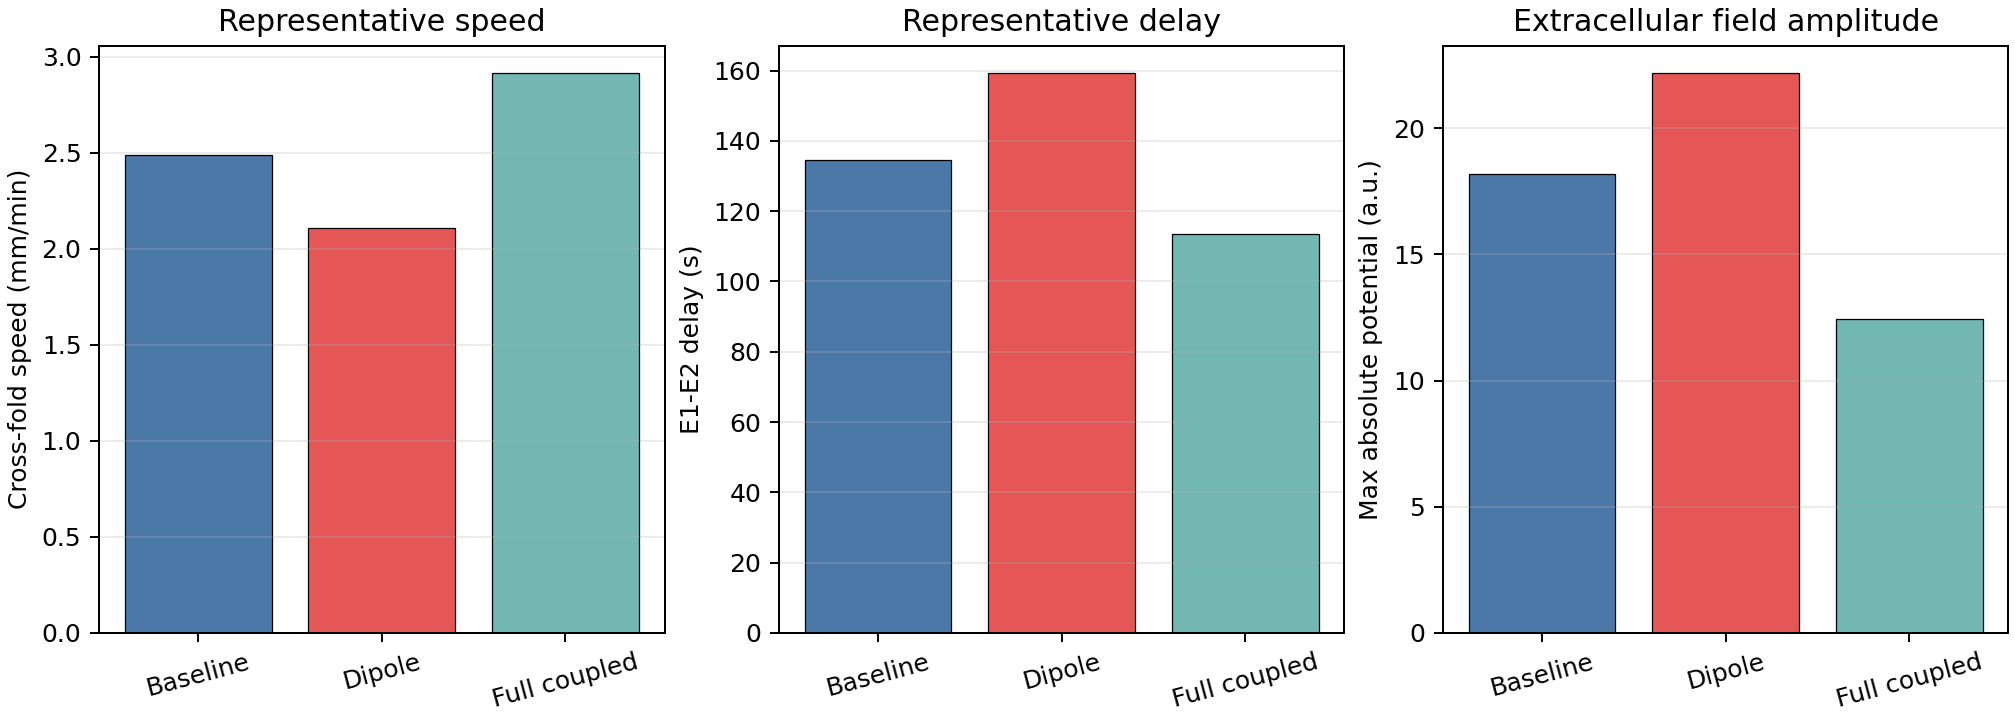
\includegraphics[width=\textwidth]{fig_mechanistic_representative_summary.png}
\caption{Representative mechanistic comparison on the folded surface. Bars show cross-fold propagation speed, cross-fold delay between the two electrode regions, and maximum absolute extracellular potential for the baseline mechanistic model, the same model with sulcal dipole alignment enabled, and the exploratory vascularly coupled extension. The primary mechanistic comparison is the paired baseline-versus-dipole contrast. The vascular extension is shown only as a sensitivity analysis because it changes the overall excitability regime.}
\label{fig:representative}
\end{figure}

\begin{table}[t]
\centering
\caption{Representative mechanistic comparison for the folded surface (fold depth 2.4~mm, $\sigma=1.5$~mm).}
\label{tab:representative}
\begin{tabular}{@{}lcccc@{}}
\toprule
Case & Speed (mm/min) & Delay (s) & Max $|\phi|$ (a.u.) & Min oxygen \\
\midrule
Baseline mechanistic & 2.488 & 134.4 & 18.20 & 1.00 \\
Dipole-aligned mechanistic & 2.106 & 159.2 & 22.17 & 1.00 \\
Full coupled sensitivity & 2.913 & 113.4 & 12.43 & 0.20 \\
\bottomrule
\end{tabular}
\end{table}

The flat control provided an internal specificity check. When fold depth was set to zero, enabling the dipole term produced no change in cross-fold speed (3.282~mm/min in both conditions) and no change in cross-fold delay (70.62~s in both conditions). Thus, the effect requires folding geometry and is not merely a numerical artifact of adding a potential equation.

\subsection{Geometry-sweep slowing}

The paired geometry sweep gave a stronger and more general version of the same result (Fig.~\ref{fig:sweep}; Table~\ref{tab:stats}). All 12 folded geometries were slower with dipole alignment, whereas the flat control again showed exactly zero effect. The mean dipole-induced slowdown was 0.243~mm/min (95\% bootstrap confidence interval 0.208--0.276~mm/min), corresponding to a mean 9.08\% reduction in speed. The associated increase in cross-fold delay was 13.46~s (95\% confidence interval 12.25--14.65~s). One-sided paired Wilcoxon signed-rank tests were significant for cross-fold speed ($p=2.44\times 10^{-4}$), cross-fold delay ($p=2.44\times 10^{-4}$), and deep-edge local speed ($p=2.44\times 10^{-3}$).

\begin{figure}[t]
\centering
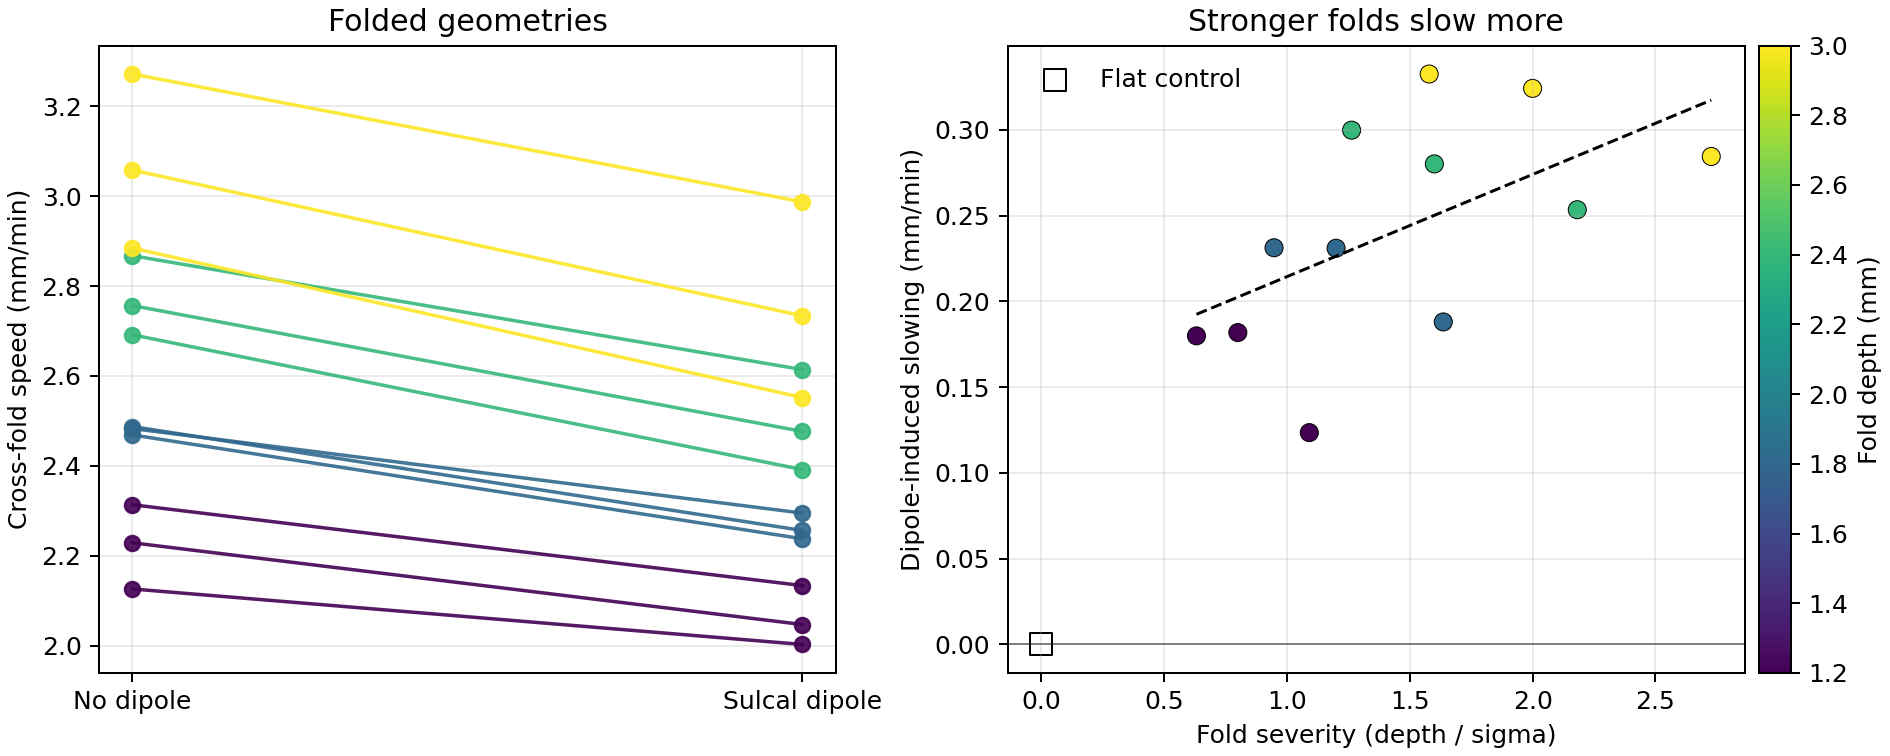
\includegraphics[width=\textwidth]{fig_mechanistic_sulcal_slowing.png}
\caption{Paired mechanistic geometry sweep. Left, each line connects the no-dipole and dipole-aligned cross-fold speeds for one folded geometry. Right, dipole-induced slowing plotted against fold severity (depth divided by width parameter $\sigma$); point color indicates fold depth. The flat control is plotted separately as a square at zero slowing. Every folded geometry slowed with dipole alignment, whereas the flat control was unchanged.}
\label{fig:sweep}
\end{figure}

\begin{table}[t]
\centering
\caption{Summary statistics for the paired folded-geometry sweep.}
\label{tab:stats}
\begin{tabular}{@{}lc@{}}
\toprule
Statistic & Value \\
\midrule
Folded geometries slower with dipole alignment & 12/12 \\
Mean speed slowdown & 0.243~mm/min \\
95\% CI for mean speed slowdown & 0.208--0.276~mm/min \\
Mean relative speed reduction & 9.08\% \\
Mean delay increase & 13.46~s \\
95\% CI for mean delay increase & 12.25--14.65~s \\
Mean deep-edge speed slowdown & 8.05~mm/min \\
Wilcoxon $p$ for speed decrease & $2.44\times 10^{-4}$ \\
Wilcoxon $p$ for delay increase & $2.44\times 10^{-4}$ \\
Wilcoxon $p$ for deep-edge slowdown & $2.44\times 10^{-3}$ \\
Spearman $\rho$ (fold depth vs slowdown) & 0.95 \\
Spearman $p$ (fold depth vs slowdown) & $2.25\times 10^{-6}$ \\
Spearman $\rho$ (depth/$\sigma$ vs slowdown) & 0.61 \\
Spearman $p$ (depth/$\sigma$ vs slowdown) & $3.58\times 10^{-2}$ \\
Flat-control slowdown & 0.000~mm/min \\
\bottomrule
\end{tabular}
\end{table}

The size of the effect increased strongly with fold depth and more moderately with fold severity. This is the pattern expected if the sulcus acts as a geometry-specific electrodiffusive bottleneck: larger folds increase the alignment between the membrane-current dipole field and the path along which extracellular drift must act to impede cross-sulcus propagation.

\subsection{The vascular extension is informative but not the primary evidence}

Turning on the exploratory vascular extension changed the representative cross-fold speed to 2.913~mm/min while simultaneously lowering oxygen to 0.20 and perfusion to 0.25 in the most affected vertices. Local edge speeds were reduced, but the global cross-fold arrival metric accelerated because the altered oxygen-dependent thresholds and pump modulation changed overall excitability. This is precisely why the vascularly coupled run is not the primary test of the dipole hypothesis: it introduces an additional physiological regime change instead of isolating the dipole term within the same ionic transport model. We therefore treat it as a sensitivity analysis showing that neurovascular coupling can interact strongly with the geometry effect, not as contradictory evidence against sulcal dipole slowing.

\section{Discussion}

The main result of this study is mechanistic rather than merely phenomenological. Within a multi-ion surface electrodiffusion model in which extracellular diffusion remains the backbone of propagation, sulcal dipole alignment produced a consistent, statistically significant slowing effect that was absent on a flat control and became stronger in deeper folds. That finding advances the project beyond earlier scalar and tensor comparison papers because it no longer depends on a prescribed attenuation field alone. Instead, the slowing arises from the interaction between geometry, membrane-current orientation, quasi-static extracellular potential, and explicit ionic drift.

The result is also well aligned with the broader CSD modeling literature. Classic and modern ionic models place extracellular K$^+$ transport, membrane fluxes, and ECS geometry at the center of the problem \citep{Tuckwell1978,Wei2014,Zandt2015}. Our model follows that logic directly by making extracellular diffusion and dynamic ECS restriction central, then adding the electrical component as a quasi-static electrodiffusive correction. In that sense, the study supports a restrained mechanistic claim: the relevant electromagnetic ingredient for CSD propagation is not wave-like radiation but the geometry-dependent extracellular potential generated by ionic charge separation and membrane currents.

The geometry specificity of the result is important. The flat control did not slow at all when the dipole term was enabled, whereas every folded geometry slowed. That makes a purely numerical explanation unlikely and instead points back to the hypothesis that sulci differ from gyri because the alignment of local dipoles and the geometry of the extracellular path are intrinsically different across those structures. The strong correlation between slowing and fold depth reinforces that interpretation.

The study also shows why vascular coupling must be handled carefully. The optional perfusion--oxygen extension did not merely add a small correction to the dipole result; it changed the overall excitability regime. That behavior is biologically plausible, but it also means that the vascular subsystem should be treated as a second-stage sensitivity analysis rather than folded into the primary claim. For a mechanistic paper centered on sulcal dipole alignment, the clean evidence is the paired comparison between the same ionic model with and without dipole alignment.

Several limitations define the scope of the present submission. First, the geometry is synthetic rather than subject-specific, so the current manuscript does not yet test dipole-induced slowing on reconstructed human cortical surfaces. Second, the electrical model is quasi-static and charge-aware, but it is still a reduced surface formulation rather than a full multidomain electrodiffusion model with explicit neuronal and glial compartments. Third, we benchmarked propagation speed and arrival-time delay, but we did not fit extracellular waveforms or direct-current shifts against experimental recordings. Fourth, the swelling state approached its model-imposed upper bound in several runs, indicating that future versions should include a more constrained volume regulation law. These limitations argue for the next steps rather than against the present conclusion: subject-specific surface bundles, waveform-level validation, and a higher-fidelity multidomain formulation would all strengthen the causal interpretation further.

Within those limits, the manuscript supports a stronger claim than the earlier tensor study. Sulcal dipole alignment is not merely compatible with CSD slowing; in a mechanistic surface electrodiffusion model it adds a significant, geometry-specific slowing term on top of extracellular diffusion, and that term scales with fold depth. That makes the current model suitable as a mechanistic hypothesis paper and a more credible basis for future patient-specific or experimentally benchmarked work.

\section*{Code availability}
The simulation code, analysis pipeline, and manuscript assets are publicly available at \url{https://github.com/squareshorts/csd-sulcus-model} and archived on Zenodo at \url{https://doi.org/10.5281/zenodo.19410880}. The mechanistic surface study reported here is implemented in \texttt{scripts/run\_surface\_mechanistic\_study.py}, with reusable model code in \texttt{src/csd\_sulcus/surface\_mechanistic.py}.

\section*{Data availability}
The processed outputs used to generate the mechanistic figures and tables are included in the repository under \texttt{outputs/surface\_mechanistic\_study/}. Manuscript-local copies of the figures are stored in \texttt{manuscript/figures/}.

\section*{Funding}
This work was financially supported by the Conselho Nacional de Desenvolvimento Cient\'ifico e Tecnol\'ogico (CNPq) under Grant No.~309589/2023-1 to A.P., and by the Coordena\c{c}\~ao de Aperfei\c{c}oamento de Pessoal de N\'ivel Superior (CAPES).

\section*{Author contributions}
A.P. conceived the study, implemented the simulations, analyzed the data, and drafted the manuscript. R.G. contributed to interpretation, critical revision, and final approval of the manuscript.

\section*{Disclosure statement}
The authors declare no competing interests.

\bibliographystyle{apalike}
\bibliography{references}

\end{document}
